\documentclass{ctexart}
\newcommand{\experimentname}{E1低温技术与高温超导研究}
\newcommand{\student}{黄振宇  \ 奎启鑫 \ 胡韵俏}
\newcommand{\Grade}{2019级}
\newcommand{\stuID}{19342043  \ 19342048 \ 19342035}
\newcommand{\previewdate}{2022.3.28}
\newcommand{\experimentdate}{4.1}
\newcommand{\reviewdate}{4.14}

\title{\experimentname}
\author{\stuID \student}
\date{\today}
\newcommand{\inlinemaketitle}{{\let\newpage\relax\maketitle}}
\renewcommand{\thesubsection}{\arabic{subsection}}

% \setCJKmainfont[BoldFont=STSongti-SC-Bold]{STSong}

\usepackage[left = 2cm , right = 2cm , top = 3cm, bottom = 3cm]{geometry}
\usepackage{amsmath}
\usepackage{listings}
\usepackage{color}


\definecolor{dkgreen}{rgb}{0,0.6,0}
\definecolor{gray}{rgb}{0.5,0.5,0.5}
\definecolor{mauve}{rgb}{0.58,0,0.82}

\lstset{frame=tb,
	language=Python,
	aboveskip=3mm,
	belowskip=3mm,
	showstringspaces=false,
	columns=flexible,
	basicstyle={\small\ttfamily},
	numbers=none,
	numberstyle=\tiny\color{gray},
	keywordstyle=\color{blue},
	commentstyle=\color{dkgreen},
	stringstyle=\color{mauve},
	breaklines=true,
	breakatwhitespace=true,
	tabsize=3
}
\usepackage{amssymb}
\usepackage{footnote}
\usepackage{yhmath}
\usepackage{float}
\usepackage{setspace}
\linespread{1.5}
\usepackage{booktabs} %\toprule
\usepackage{array}% tabular using m{2cm}, m , vertical alignment
\usepackage{titlesec}
\usepackage{appendix}
\usepackage{graphicx}
\usepackage{wrapfig}
\usepackage{subcaption}
\usepackage{tikz}
%定义插入 TikZ 作图命令
\newcommand{\inputtikzfigure}[1]{\input{#1.tex}}
\usepackage{esint} %积分
\usepackage{siunitx}%单位
\usetikzlibrary{arrows.meta}
\usepackage[T1]{fontenc}
\usepackage{tabularx}
\usepackage{pdfpages}

%定义罗马数学
\usepackage{mathrsfs}%使用花体字 命令\mathscr
\usepackage[bookmarks=true,colorlinks=true]{hyperref} %超链接
\hypersetup{linkcolor=[rgb]{1,0.27,0}, bookmarksopen = true}% 更多设置请查阅: texdoc hyperref

\usepackage[inline]{enumitem} % 编号
% 新列表 (间距较小):
\newlist{conditionlist}{enumerate}{2}
\setlist[conditionlist,1]{topsep = 0pt, itemsep = 0pt, parsep = 0pt,%
	label=\arabic*), leftmargin=2\parindent}
\setlist[conditionlist,2]{topsep = 0pt, itemsep = 0pt, parsep = 0pt,%
	label=\alph*), leftmargin=3\parindent}

\usepackage{listing} % 用于展示代码

\DeclareMathOperator{\tg}{tg}
\DeclareMathOperator{\ctg}{ctg}
\DeclareMathOperator{\arctg}{arctg}
\DeclareMathOperator{\sh}{sh}
\DeclareMathOperator{\ch}{ch}

% 页眉, 表头信息

\usepackage{fancyhdr}
\pagestyle{fancy}
\fancyhf{}
\cfoot{\thepage}
\lhead{中山大学物理与天文学院基础物理实验报告}
\chead{$\qquad\qquad\quad$\student}
\rhead{\experimentname}


\usepackage{amsthm}
\usepackage[framemethod=tikz]{mdframed}

\definecolor{ocre}{RGB}{243,102,25}
\definecolor{mygray}{RGB}{243,243,244}
\definecolor{myblue}{RGB}{18,24,176}

\newcommand*\mymathbox[1]{%
	\fcolorbox{ocre}{mygray}{\hspace{1em}#1\hspace{1em}}}

\newtheoremstyle{ansstyle}
{\topsep}
{\topsep}
{\normalfont}
{}
{\sffamily\bfseries}
{\\}
{.5em}
{{\color{ocre}\thmname{#1}~\thmnumber{#2}}\thmnote{\,--\,#3}}%

\theoremstyle{ansstyle}
% \theoremstyle{break}  
\newmdtheoremenv[
backgroundcolor=mygray,
linecolor=ocre,
leftmargin=0pt,
innerleftmargin=10pt,
innerrightmargin=10pt,
]{ans}{Answer}[section]

\newcommand{\infotable}{%
	\begin{center}
		\begin{tabular}{|p{1.49cm}<{\centering}|p{1.49cm}<{\centering}|p{1.49cm}<{\centering}|p{1.49cm}<{\centering}|p{1.49cm}<{\centering}|p{1.49cm}<{\centering}|p{1.49cm}<{\centering}|p{1.49cm}<{\centering}|}
			\specialrule{0em}{0.3cm}{0cm}
			\hline
			\multicolumn{2}{|c|}{\LARGE 预习实验} & \multicolumn{2}{c|}{\LARGE 实验记录}& \multicolumn{2}{c|}{\LARGE 分析讨论} & \multicolumn{2}{c|}{\LARGE 总成绩} \\
			\hline
			&&&&&&& \\
			\hline
			\specialrule{0em}{0.3cm}{0cm}
		\end{tabular}
	\end{center}%
}

\newcommand{\previewdata}{% 总的信息
	\begin{center}
		\begin{tabular}{|p{1.5cm}|p{4.5cm}|p{4cm}|p{3.65cm}|}
			\hline
			{\large 专业}:  & {\large 物理学}    & {\large 年级: }    & {\large \Grade} \\
			\hline
			{\large 姓名: } & \multicolumn{3}{c|}{\large \student} \\
			\hline
			{\large 学号: }  & \multicolumn{3}{c|}{\large \stuID} \\
			\hline
			{\large 日期: } & {\large \previewdate} & {\large 教师签名: } & \\
			\hline
			\specialrule{0em}{0.6cm}{0cm}
		\end{tabular}
	\end{center}%
}

\newcommand{\experimentdata}{% 实验记录
	\begin{center}
		\begin{tabular}{|p{2cm}|p{4cm}|p{4cm}|p{4cm}|}
			\hline
			专业:  & 物理学 & 年级:  & \Grade \\
			\hline
			姓名:  & \multicolumn{3}{c|}{\student} \\
			\hline 
			学号:  & \multicolumn{3}{c|}{\stuID} \\
			\hline
			日期:  & \experimentdate & & \\
			\hline
			评分:  &   & 教师签名: & \\
			\hline
		\end{tabular}
	\end{center}%
}

\newcommand{\reviewdata}{% 分析与讨论
	\begin{center}
		\begin{tabular}{|p{2cm}|p{4cm}|p{4cm}|p{4cm}|}
			\hline
			专业: & 物理学 & 年级:  & \Grade \\
			\hline
			姓名:  & \multicolumn{3}{c|}{\student} \\
			\hline 
			学号:  & \multicolumn{3}{c|}{\stuID} \\
			\hline
			日期: & \reviewdate & & \\
			\hline
			评分: & & 教师签名: & \\
			\hline
		\end{tabular}
	\end{center}%
}

\newcommand{\me}{\mathrm{e}} % 自然对数的底
\newcommand{\mi}{\mathrm{i}} % 虚数单位
\newcommand*{\basis}[1]{\hat{\boldsymbol{#1}}} % 基底
\newcommand*{\bv}{\boldsymbol} % 向量加粗
\newcommand*{\id}{\mathrm{id}} % 单位映射
\newcommand*{\IFF}{\;\leftrightarrow\;} % 充要条件
\newcommand*{\dif}[1][1]
{\if#11%
	\mathop{}\!\mathrm{d}%
	\else%
	\mathop{}\!\mathrm{d}^#1
	\fi} % 微分算子d
\newcommand*{\diff}[3][1]
{\if#11%
	\frac{\mathrm{d} #2}{\mathrm{d} #3}% 导数\diff{y}{x}
	\else%
	\frac{\mathrm{d}^{#1} #2}{\mathrm{d} #3^{#1}}% n阶导数\diff[n]{y}{x}
	\fi}
\newcommand*{\pdiff}[3][1]
{\if#11%
	\frac{\partial #2}{\partial #3}% 偏导数\pdiff{y}{x}
	\else%
	\frac{\partial^{#1} #2}{\partial #3^{#1}}% n阶偏导数\pdiff[n]{y}{x}
	\fi}
\newcommand*{\deltadiff}[3][1]
{\if#11%
	\frac{\delta #2}{\delta #3}% 导数\diff{y}{x}
	\else%
	\frac{\delta^{#1} #2}{\delta #3^{#1}}% n阶导数\diff[n]{y}{x}
	\fi}
\newcommand*{\atpoint}[2]
{
	\left.
	{#1}
	\right\vert_{#2}
}

\newcommand{\showfig}[2][14.5cm]{
	\begin{figure}[H]
		\centering
		\includegraphics[width=#1]{#2}
		%对于A4大小的图片, 不要比这个尺寸大
		% \caption{<CAPTION>}
	\end{figure}
}

\newcounter{instruCounter}
\setcounter{instruCounter}{0}
\newcommand{\instrument}[3]{%
	\stepcounter{instruCounter}\theinstruCounter &%
	#1 &%
	#2 &%
	#3 \\
	\hline
}

\lstloadlanguages{Python}
\lstset{language=Python,commentstyle=\scriptsize}
\begin{document}
	\sisetup{separate-uncertainty, range-phrase=\textup{--}}
	\noindent
	\renewcommand\arraystretch{1.8}
	\infotable
	
	% \noindent
	\renewcommand\arraystretch{1.3}
	\previewdata
	
	\inlinemaketitle
	\tableofcontents
	
	\subsection{实验报告注意事项}
	
	\begin{enumerate}
		\item 实验报告由三部分组成: 
		\begin{enumerate}
			\item \textbf{预习报告}: 
			(提前一周) 认真研读\underline{\textbf{实验讲义}}, 弄清实验原理;实验所需的仪器设备、用具及其使用 (强烈建议到实验室预习) , 完成讲义中的预习思考题;了解实验需要测量的物理量, 并根据要求提前准备实验记录表格 (由学生自己在实验前设计好, 可以打印) . 预习成绩低于10分 (共20分) 者不能做实验. 
			\item \textbf{实验记录}: 
			认真、客观记录实验条件、实验过程中的现象以及数据. 实验记录请用珠笔或者钢笔书写并签名 ({\color{red}用铅笔记录的被认为无效}) . {\color{red}保持原始记录, 包括写错删除部分, 如因误记需要修改记录, 必须按规范修改. } (不得输入电脑打印, 但可扫描手记后打印扫描件) ;离开前请实验教师检查记录并签名. 
			\item \textbf{分析讨论}: 
			处理实验原始数据 (学习仪器使用类型的实验除外) , 对数据的可靠性和合理性进行分析;按规范呈现数据和结果 (图、表) , 包括数据、图表按顺序编号及其引用;分析物理现象 (含回答实验思考题, 写出问题思考过程, 必要时按规范引用数据) ;最后得出结论. 
		\end{enumerate}
		\underline{实验报告}就是预习报告、实验记录、和数据处理与分析合起来, 加上本页封面. 
		\item 每次完成实验后的一周内交\underline{实验报告}. 
		\item 除实验记录外, 实验报告其他部分建议双面打印. 
	\end{enumerate}
	
	% 预习报告 
	
	\addcontentsline{toc}{section}{预习报告}
	\stepcounter{section}
	\section*{\experimentname 预习报告}
	
	\subsection{实验目的}
	
	\begin{enumerate}
		\item 学习基本的低温技术,掌握深冷温区的获得和测量方法
		\item 掌握超导电性的两个基本特征:零电阻和迈斯纳效应,认识磁场对超导临界温度的影响,对宏观量子化有一个初步的认识;学习多变量对研究对象影响的研究方法
		\item 学习将弱信号测量技术应用于超导转变的测量:直流四引线法用于零电阻特性测量实验内容 1),交流磁化率用于迈斯纳效应测量(2);学习为测量提供磁场条件
		\item 复习巩固信号提取方法之“本底扣除”,包括硬件设计中的物理扣除和数据处理时的数值扣除
		\item 巩固和加深数据采集系统的认识,学习用 LabView 管理实验
	\end{enumerate}
	
	\subsection{实验用具}
	\begin{table}[H]
		\begin{center}
			\begin{tabular}{|c|c|c|m{12cm}|}
				\hline
				编号 & 仪器用具名称 & 数量 & 主要参数 \\
				\hline
				\instrument{循环制冷剂}{1}{} % \instrument{名称}{数目}{参数}
				\instrument{高温超导陶瓷}{1}{$YBa_2Cu_3O_7$-?陶瓷样品}
				\instrument{磁场系统}{1}{EM3 电磁铁+ P10-40 电源}
			\end{tabular}
			%\caption{<Caption>}
		\end{center}
	\end{table}
	
	
	
	\subsection{原理概述}
	见实验讲义
	
	\subsection{实验前思考题}
	\subsubsection{实验目的一}
	\begin{enumerate}
		\item 深低温系统为什么要抽真空?真空度要求多高?
		\paragraph{答:}传热有三种方式:热传导,对流与热辐射。抽真空可以避免热对流的影响
		\item 真空泵产生一定的噪声,在达到真空要求后,是否可以关真空泵?关真空泵前,是
		否要先关真空阀门?
		\paragraph{答:}真空泵只能使得样品处于一个较为粗糙的真空环境,需要通过循环制冷机持续工作达到更高的真空度。而此时循环制冷机起到分子泵的作用。关闭真空泵可以减去真空泵噪声对实验结果的影响。关闭真空泵前,要关闭真空阀门。
		\item 为什么要安装屏蔽罩(防辐射屏)? 屏蔽罩用哪一类材料最好?
		\paragraph{答:}若当在物体与环境之间插入一低温物体作为防辐射屏,则从防辐射屏到物体之间的漏热比从环境的直接漏大大降低。即使在物体与环境之间插入一物体作为防辐射屏,并让它自然达到热平衡,即从环境对防辐射屏的净漏等于从防辐射屏到低温物体的净漏热,则从环境到低温物体的净漏热减半。
		$$\Delta Q=\sigma (T_{E}^4-T_{M}^4)=\sigma (T_{M}^4-T_{L}^4)=\frac{1}{2}\sigma(T_{E}^4-T_{L}^4)$$
		\item 请估计直径为 12mm、长为 100mm,温度为 4K 的恒温器在无防辐射屏时的漏热约为多少?在采用
		一层防辐射屏后,其与环境之间的辐射漏热减少了多少? 如果将防辐射屏的温度降到液氮温度(77K),则该防辐射屏的辐射漏热又为多少?
		\paragraph{答:}由斯特潘玻尔兹曼定律,辐射传热与辐射体绝对温度的 4 次方成正比。在方便计算的情况下,将恒温器
		和环境看作理想黑体,且假设环境温度为 300k。由直径 12mm 和长 100mm 温度为 4K 的恒温器在无防辐射屏时的漏热为的圆柱可计算得到表面积为。
		$$S=2\pi r \cdot L+2\pi r^{2}=1272\pi mm^{2}$$
		单位时间漏热
		$$\Delta Q=S \cdot \sigma(T_{E}^4-T_{L}^4)=1.731W$$
		使用防辐射屏后,漏热平衡时漏热减半。
		$$\Delta Q^{'}=\frac{1}{2} S \cdot \sigma(T_{E}^{4}-T_{L}^{4})=0.866W $$
		将防辐射屏温度降到 77K,则辐射屏单位时间漏热
		$$\Delta Q=S\cdot \sigma(T_{M}^{4}-T_{l}^4)=7.96\times 10^{-3}W$$
		\item 铂电阻温度计位置不在样品旁边,有什么因素会影响样品温度偏离温度计的温度? 偏离有多大?能否通过建模进行定量分析
		\paragraph{答:}固体热传导:
		$$\dot{Q}=\kappa \Delta T\frac{S}{L}$$
		$$\Delta T=\frac{Jl}{\kappa}$$
		其中$J=\frac{\dot{Q}}{S}$,分析易得,热流密度J与样品和铂电阻的距离L以及样品和电阻的材料导热率$\kappa$都能影响两者温差$\Delta T$
		当等待时间较长,系统趋于稳态,热流密度 J 趋于零,则温差也趋于零。所以温度测量的效率和准确不能兼顾。\\
		若导热性极好,热导率κ趋于无穷,则温差为零,所以最好的办法是尽量将铂电阻安装在样品上或者尽量靠近样品。
	\end{enumerate}
	\subsubsection{实验目的3磁场}
	\begin{enumerate}
		
		\item 高磁场下电磁铁长时间工作会导致线圈温度升高,如何在满足实验需求的同时,使线圈`
		\paragraph{答:}为了避免电磁铁长时间工作导致线圈温度升高,在做实验时,只有当需要用到磁场时才将磁场打开,其余时间把电磁铁磁场关闭,让其散热冷却。让电磁铁间歇式工作可以让磁场处于工作的较佳状态
		\item 本实验中样品位置的磁场与霍尔探头测量的磁场有多大的偏差?如何校正?校正时电磁铁电源能用“磁场模式”吗?为什么?
		\paragraph{答:}可知载流I的圆形导线在其轴线上(距圆心x处)的磁场会有
		$$B=\frac{\mu_{0}}{2}\cdot \frac{IR^{2}}{(R^{2}+x^{2})^{\frac{3}{2}}}$$
		所以总磁场为
		$$B=\frac{\mu_{0}}{2}\cdot (\frac{1}{(R^{2}+(x_{0}-x)^{2})^{3/2}}+\frac{1}{(R^{2}+(x_{0}+x)^{2})^{3/2}})$$
		得到泰勒一阶展开项为$$B=-\frac{3\mu_{0}IR^{2}x_{0}x}{(R^{2}+x_{0}^{2})^{5/2}}$$
		将x为霍尔探头到线圈中点的距离代入可算得偏差。当样品位置和控制点位置确定时,两者相对磁场关系也确定,通过特斯拉计测量磁隙不同位置,得到样品位置和传感器位置的磁场关系,最后放入样品测量磁隙位置磁场算出样品位置的磁场。由于磁场模式通过特斯拉计反馈控制,未达到磁场会一直增加电流,所以需要改用电流模式及。
		\item 如果采用“电流模式”加磁场,电磁铁的剩磁有多大?实验中可以消除剩磁到什么水平?
		\paragraph{答:}由于磁畴运动不可避免地受到阻碍,造成铁磁材料的“磁滞”现象,电磁铁磁隙内的磁场(或磁化强度)并不与外加电流形成严格的对应关系。需要实验具体测量。
		\item 如果采用“磁场模式”加磁场,会有剩磁问题吗?
		\paragraph{答:}不会有剩磁问题,因为该模式是通过特斯拉计测量磁场值反馈控制,从而获得所需磁场,且该模式自带自动消磁的功能。
		
		
	\end{enumerate}
	\subsubsection{实验目的 3 之电磁测量}
	
\begin{enumerate}	
	
	\item 外加磁场与电流方向的夹角不同,洛伦兹力不同,从而超导体的磁流阻大小不同。针对研究磁场(矢量)对超导转变的影响,写出你的实验方案
	\paragraph{答:}原理:当外加磁场与电流平行时,洛伦兹力为零,磁流阻最小;而当它们相互垂直时,洛伦兹力最大,磁通会在洛伦兹力的作用下运动,从而产生电压降,磁流阻最大。\\
	设计:在直流四引线测电阻方法的装置,先根据基础实验得到的某一温度下比下临界磁场强度稍大的磁场强度值,调节装置先降温使其变为超导态,再加磁场使其进入混合态,此时施加直流电流测得一个电阻值,其他条件不变,将固定样品的装置水平旋转 90$^\circ$ 、 180$^\circ$ 分别测此时电阻值的变化情况。
	\item 测量交流磁化率的实验装置上的两个已经连接好的次级线圈不能做到完全对称, 测试人
	员并不知道单个线圈的输出电压是多少, 如何判断次级线圈是以抵消本底的方式连接?
	\paragraph{答:}用回形针分别插入两个线圈,输入信号反相则反接,同相则正接
	\item 交流信号包含幅值(R)和相位($\theta$),或实部和虚部,由于实际制备时两个次级线圈不可能做到完全对称从而抵消本底信号,那么
	\begin{enumerate}
		\item 由此造成的本底信号(含幅值和相位)可以被扣除吗
		\paragraph{答:}\begin{figure}[H]
			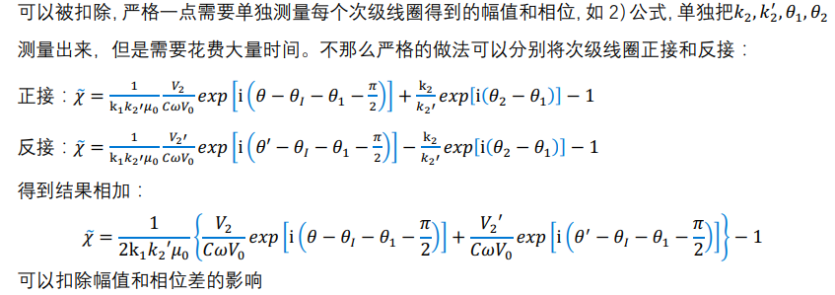
\includegraphics[width=0.8\linewidth]{./be/1}
		\end{figure}
		\item 由两对线圈完全对称假设而推出的式(E1- 18)会变成怎样?请推导
		\paragraph{答:}\begin{figure}[H]
			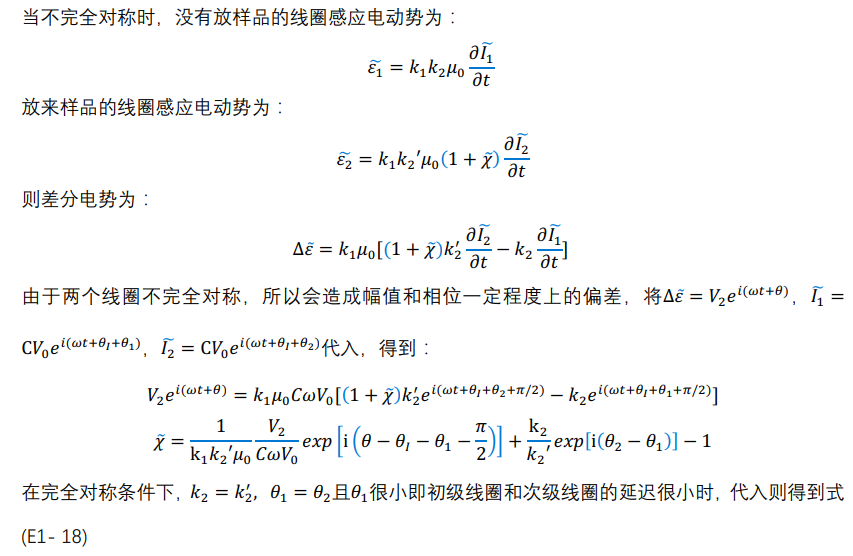
\includegraphics[width=0.8\linewidth]{./be/2}
		\end{figure}
		\item 实部与虚部的区分依赖于相位差测量,如何扣除交流磁化率测量系统的相位差本底?(如下图参考双
		通道锁相放大器微小阻抗测量实验中的用取样电阻获得初级 线圈电流相位$\theta_{I}$)
		\paragraph{答:}\begin{figure}[H]
			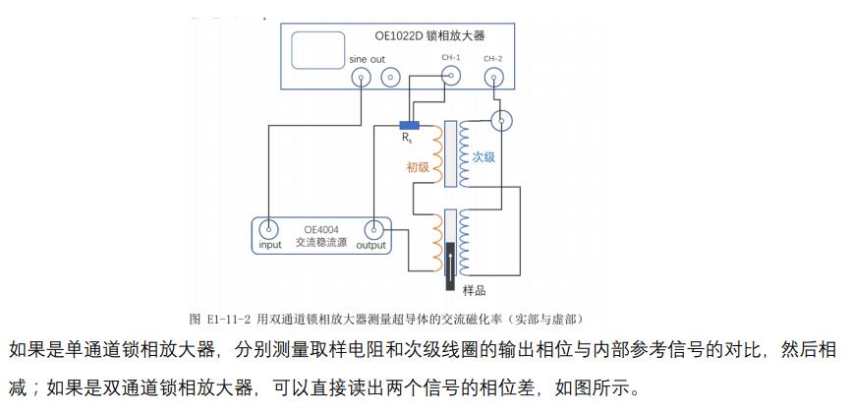
\includegraphics[width=0.8\linewidth]{./be/3}
		\end{figure}
	\end{enumerate}
	
	\item 如何对磁化率定标?实部或虚部能同时定标吗?
	
	\paragraph{答:}通过已知磁化率的标样可以对系数定标。将标样放入样品槽中,设定一个确定的频率值,后续实验不改变频率值,然后通过锁相放大器的相位读数,得到$\frac{V_{2}}{C\omega V_{0}}cos(\theta-\theta_{I}-\frac{\pi}{2})$和$\tilde{\chi}$的关系,其比值就是互感系数。由于实部和虚部的系数一致,所以两者可以同时定标。
	\paragraph{答:}
	\item 交流互感一级线圈的电阻为 34 ,对于稳流源的最大输出 0.1A,所产生的焦尔热为 0.34W,它对样品温度产生多大的影响?有什么方法降低该影响?(提示,设线圈与恒温器的接触热阻为 20K/W)
	\paragraph{答:}$0.34\times 20=6.8K$
	减少影响的方法有:\begin{enumerate}
		\item 减少一级线圈与样品的接触面积,减慢热量传导的过程;
		\item 将测温的 pt1000 安装到更靠近样品的位置,减少测温误差
	\end{enumerate}
	\item 线圈架用材料做合适?为什么不能用金属? (提示:应用电磁学中的电磁感应知识。)
	\paragraph{答:}用塑料做较为合适,使用金属会在磁场作用下产生感应电流,进而产生磁场,造成磁场分布的不均匀性,影响实验结果。
	\item 互感线圈为何要用锰铜丝绕制?如果用纯铜漆包线绕制会如何?
	\paragraph{答:}低温对互感器带来的最大问题是对互感器结构和绝缘的破坏。如常规塑料或普通环氧制作的互感器在低温下回因为热胀冷缩而开裂,影响测量的精度,甚至损坏互感器;常规绝缘材料在低温下可能出现开裂,导致绝缘破坏,威胁到整个测试系统的安全。
\end{enumerate}

\newpage

\experimentdata

\addcontentsline{toc}{section}{实验记录}
\stepcounter{section}
\section*{\experimentname 实验记录}
外磁场如何影响超导转变时磁化率随温度的关系包括($T_c$)和抗磁性?
\subsection{科学问题选题}
\textbf{
	\begin{enumerate}
		\item 超导现象是否历史相关(如先降温后加场或先加场后降温)?
		\item 外磁场如何影响超导转变时磁化率随温度的关系[包括( $T_{c}$)和抗磁性(($\tilde{\chi}$) ]?
\end{enumerate}}
\subsection{实验内容、步骤、结果}
\subsubsection{题一步骤}
\begin{enumerate}
	\item 选定两个态,在这里我们选定的态为(85K, 0kGs)和(79K, 2kGs)。然后分别沿着两条路径,从第一个态转变到第二个态
	\item 先从 85K 转变到 79K,然后再增加磁场到 2kGs。温度的步进是 1K,然后磁场的步进是 0.5kGs。
	\item  85K 下,先增加磁场到 2kGs,然后再逐步降温到 79K。 步进同上。
\end{enumerate}
我们想要验证的是,无论沿着哪一条路径,样品最终抵达的态的参数(R,$\theta$)是相同的。也就是说,我们要验证
的态是热力学态,因为热力学态的转变与路径无关。
\subsubsection{题二步骤}
\begin{enumerate}
	\item 控温至 78K 左右
	\item 设置电流为 50mA,外加磁场为 1kGs。
	\item  记录每次改变温度并稳定后的测量电压,正反各一次
	\item 改变外加磁场分别为 2kGs 和 3kGs,重复步骤 1、 2、 3、 4
	\item 改变设置电流分别为 100mA, 150mA, 200mA,重复步骤 1、 2、 3、 4
\end{enumerate}
\subsection{实验过程遇到的问题}
\paragraph{}第一周实验中,样品处温度通过PT1000电阻值获得,而控温仪(冷指温度)与样品处温度不同。实验中控温仪数值降到一定程度时,PT1000显示电阻计算得到的样品实际温度仍然过大(超过100K),故无法观察到转变温度,且降不到指定温度。\\
解决方法:调节锁相放大器样品处线圈电流从0.5A至0.1A,使线圈产生的焦耳热下降。(此解决方式缓解了一些,但降温仍然十分缓慢。)第二次实验时,问题得到解决:交流电流源输出电流过大,更换电流源后实验正常。
  \paragraph{}第二周实验时,在PT1000温度显示正常的情况下,仍无法观察到临界现象,因此怀疑是样品有问题。
  \paragraph{}第三次实验,更换样品后,一切实验正常。(但被替换下来的样品能观察到磁悬浮,理论上样品没有问题。)

\newpage

% 分析和讨论

\reviewdata

\addcontentsline{toc}{section}{分析与讨论}
\stepcounter{section}
\section*{\experimentname 分析与讨论}

% \setcounter{section}{0}

\subsection{分析与讨论}
\subsubsection{实验操作分析}
\paragraph[short]{磁场标定}  已知两线圈中间有空间分布的磁场,且高斯计无法直接测得样品所在位置的磁场大小,于是采用先定标磁场
得到边缘磁场与中央磁场的关系的方法
\begin{table}[H]
\centering
\begin{tabular}{@{}llll@{}}
\toprule
电流(A)  & 1     & 2     & 3     \\ \midrule
中心(kG) & 0.495 & 0.261 & 0.104 \\
边缘(kG) & 0.547 & 0.28  & 0.121  \\ \bottomrule
\end{tabular}
\end{table}
我们以边缘磁场与中心磁场关系用采用最小二乘做线性拟合会得到直线的斜率和截距,如下图所示。
\\
实验得到,边缘磁场与中心磁场呈线性关系,边缘磁场的 1.1 倍为中心磁场的大小
\begin{figure}[H]
	\centering
	\caption{标定磁场拟合图像}

	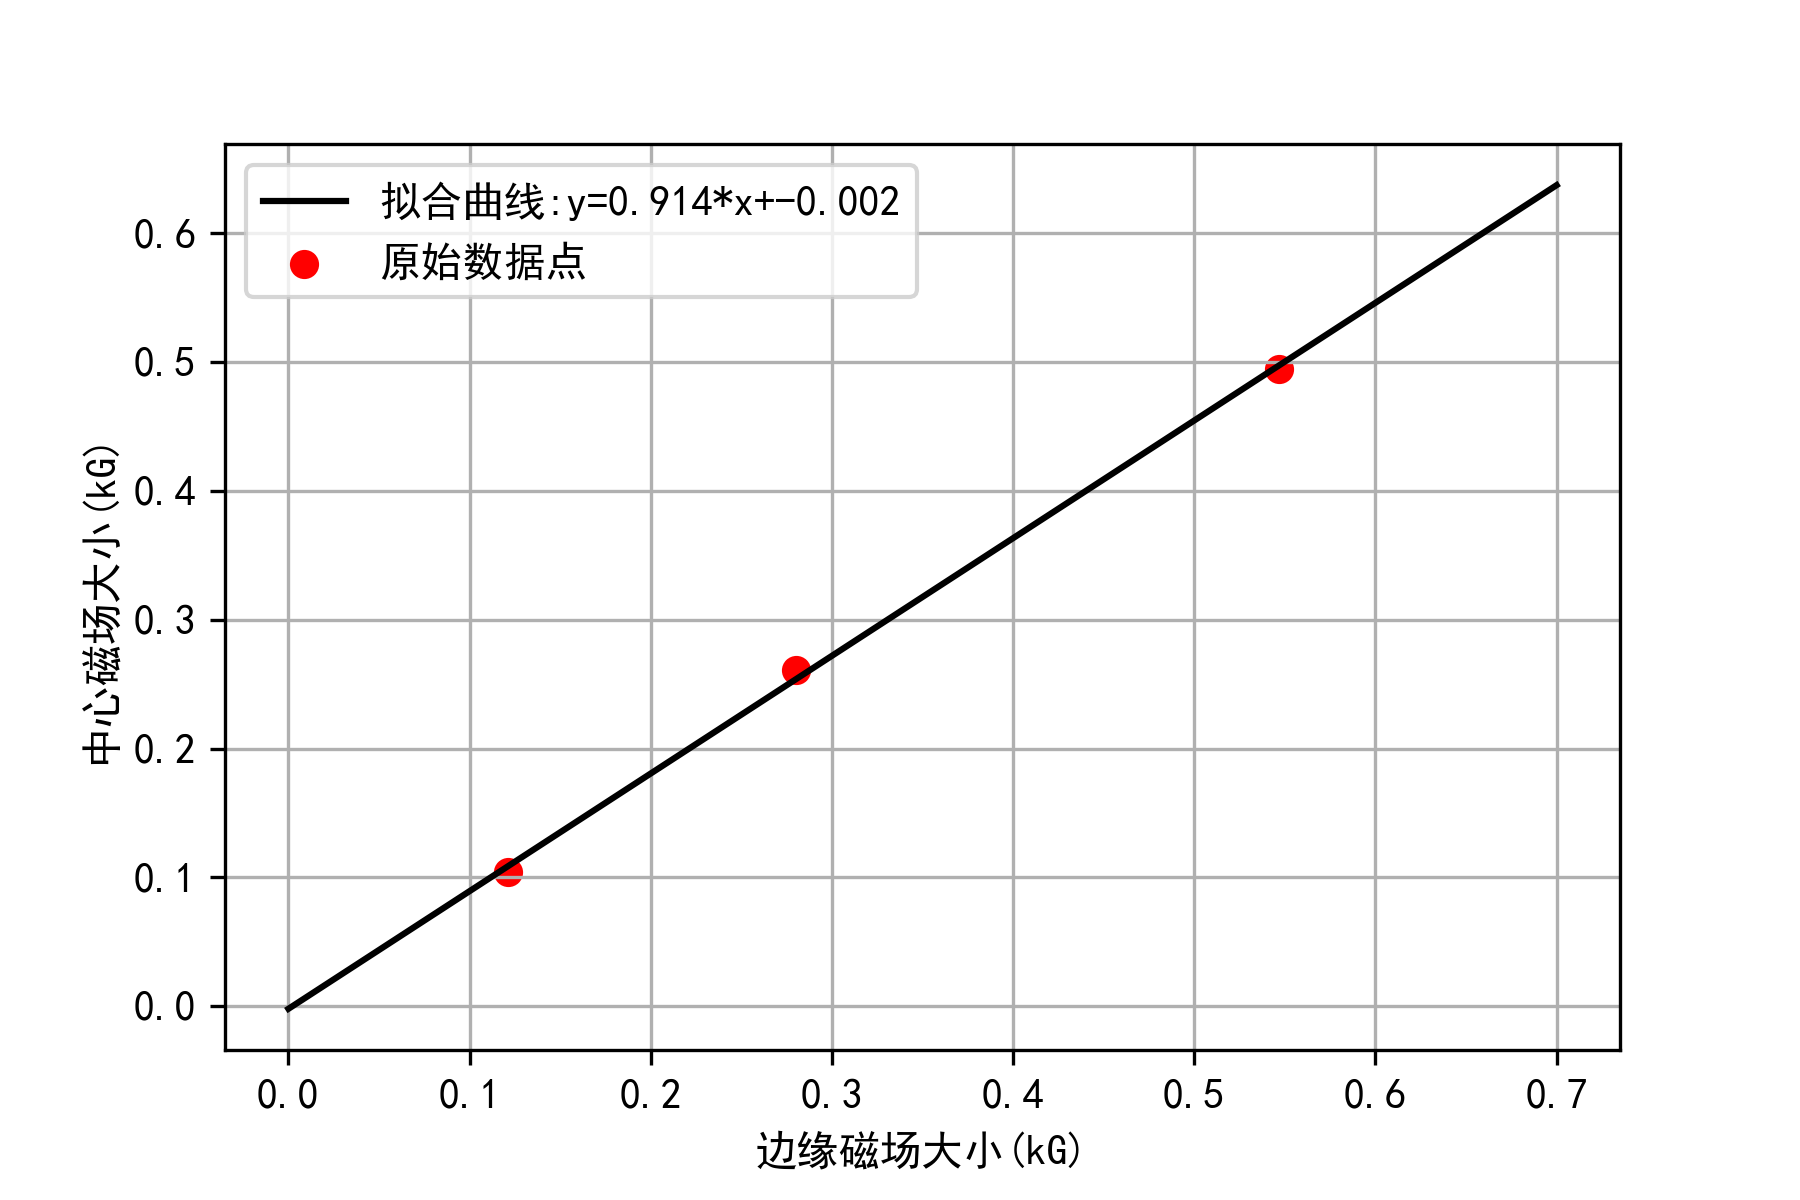
\includegraphics[width=0.75\linewidth]{./png/q1.png}
\end{figure}
\paragraph{磁化率与温度变化关系(升温与降温)} 磁化率无法标定。磁化率表征材料对外加磁场(变化)的响应,对外加磁场响应的定义为直流磁化率$ \chi $ ,
对外加磁场变化响应的为交流磁化率$ \widetilde{\chi}  $ 。 对于小振幅交变磁场, 交流磁化率$ \widetilde{\chi}  $反映的是材料磁
化曲线的斜率,亦称微分磁化率我们会有公式
\begin{equation}
    \centering
	M=\chi H
\end{equation}
$ \chi $为磁化率 
\begin{equation}
    \widetilde{\chi} =\frac{\partial M}{\partial H} 
\end{equation}
交流磁化率通常通过一对缠绕在一起的互感线圈来测量:负责产生磁场的线圈称为初级
线圈,负责检测样品磁响应的线圈称为次级线圈。单个次级线圈感应的电动势与线圈内部磁
感应强度 B(t)的变化率成正比,
因此用V2与温度的关系代替磁化率与温度的变化关系,可以得到转变温度。对于温度,我们记录了Pt1000的阻值变化情况,通过查表可得对应的电阻与温度(K)\\
\paragraph{信号处理} 对于锁相放大器采集的信号,我们发现它在一些温度下的信号出有着不正常的跳动(指R值数据),我们认为是
锁相放大器的时间常数或者滤波微分积分设置不当等一系列采样问题导致的数据波动,为了剔除这些噪音,我们采用了S-G滤波来进行数据处理。
\begin{figure}[H]
	\centering
		\begin{minipage}[t]{0.48\linewidth}
			\centering
			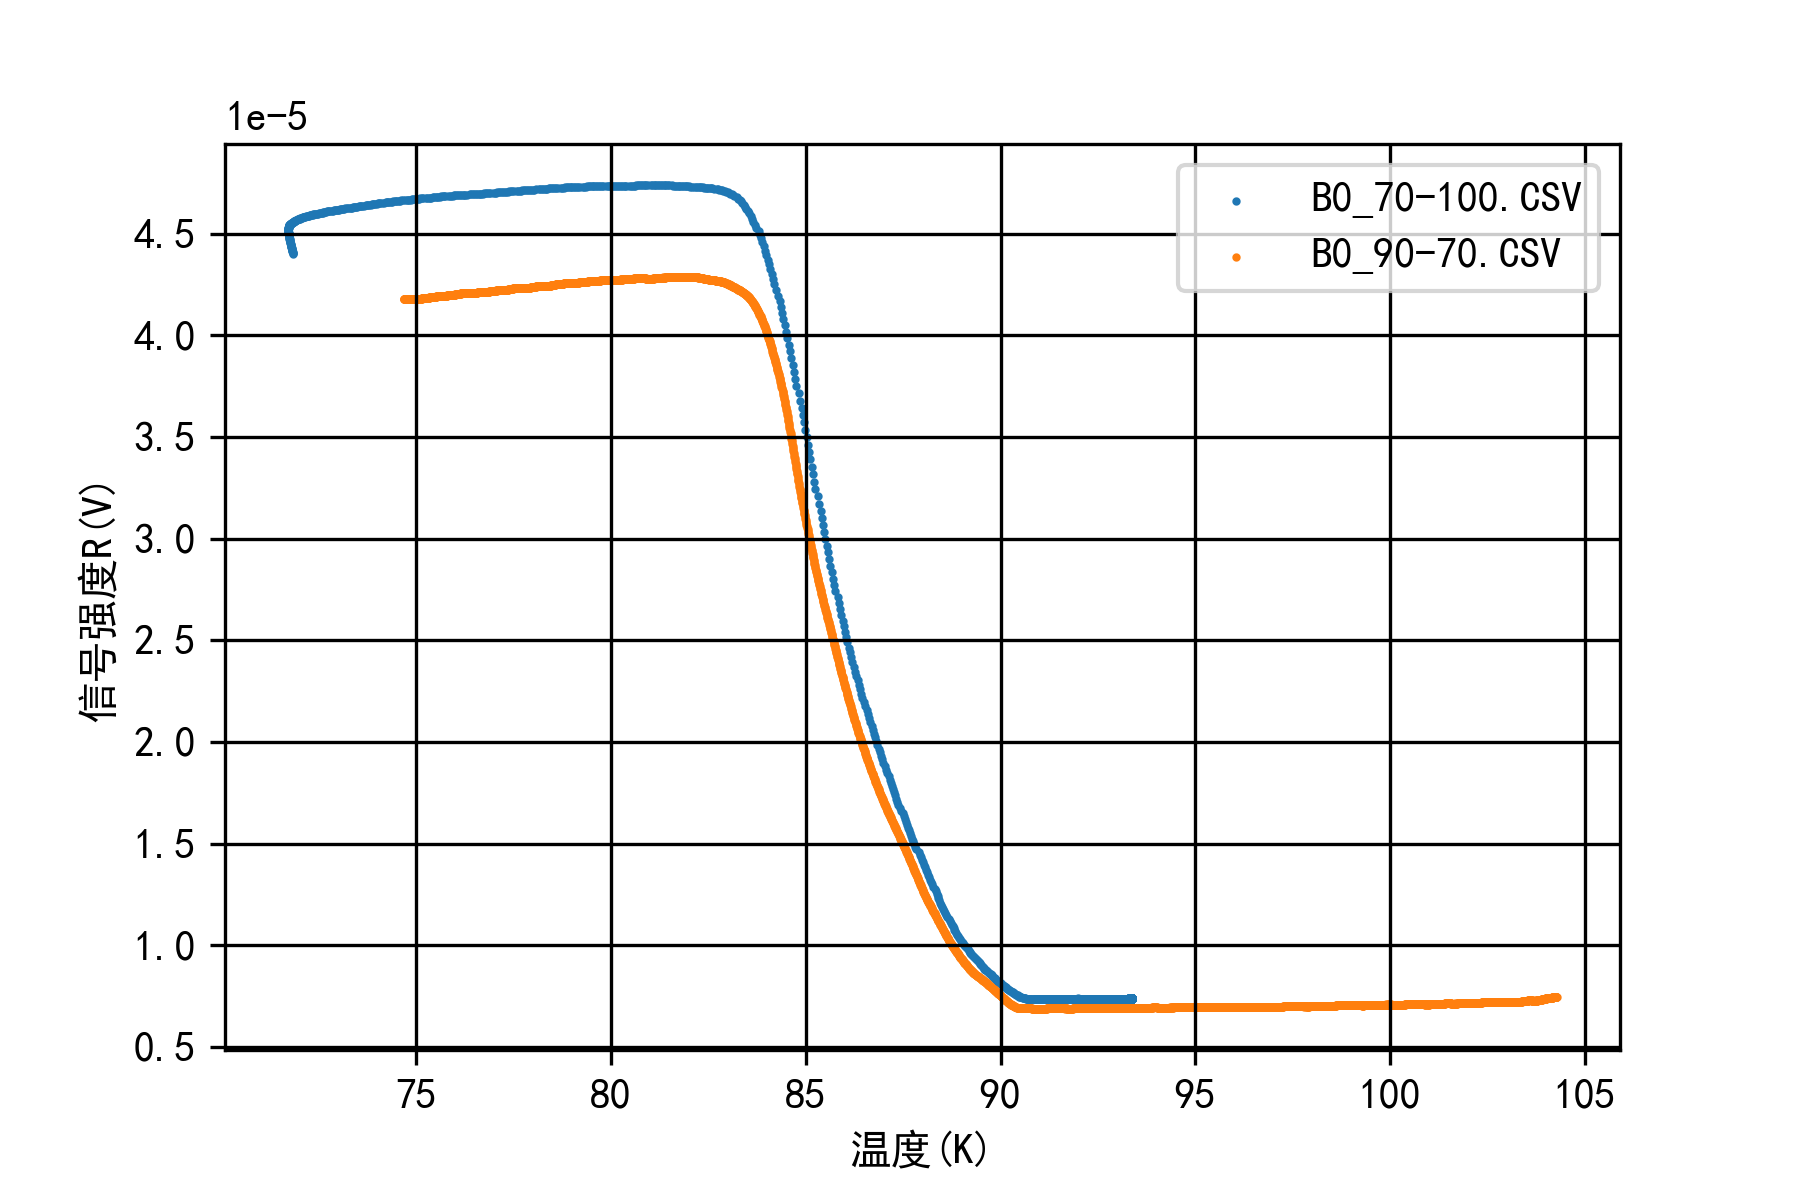
\includegraphics[width=0.9\linewidth]{./png/2.png}
			\caption{设置电流为0A}
		\end{minipage}
		\begin{minipage}[t]{0.48\linewidth}
			\centering
			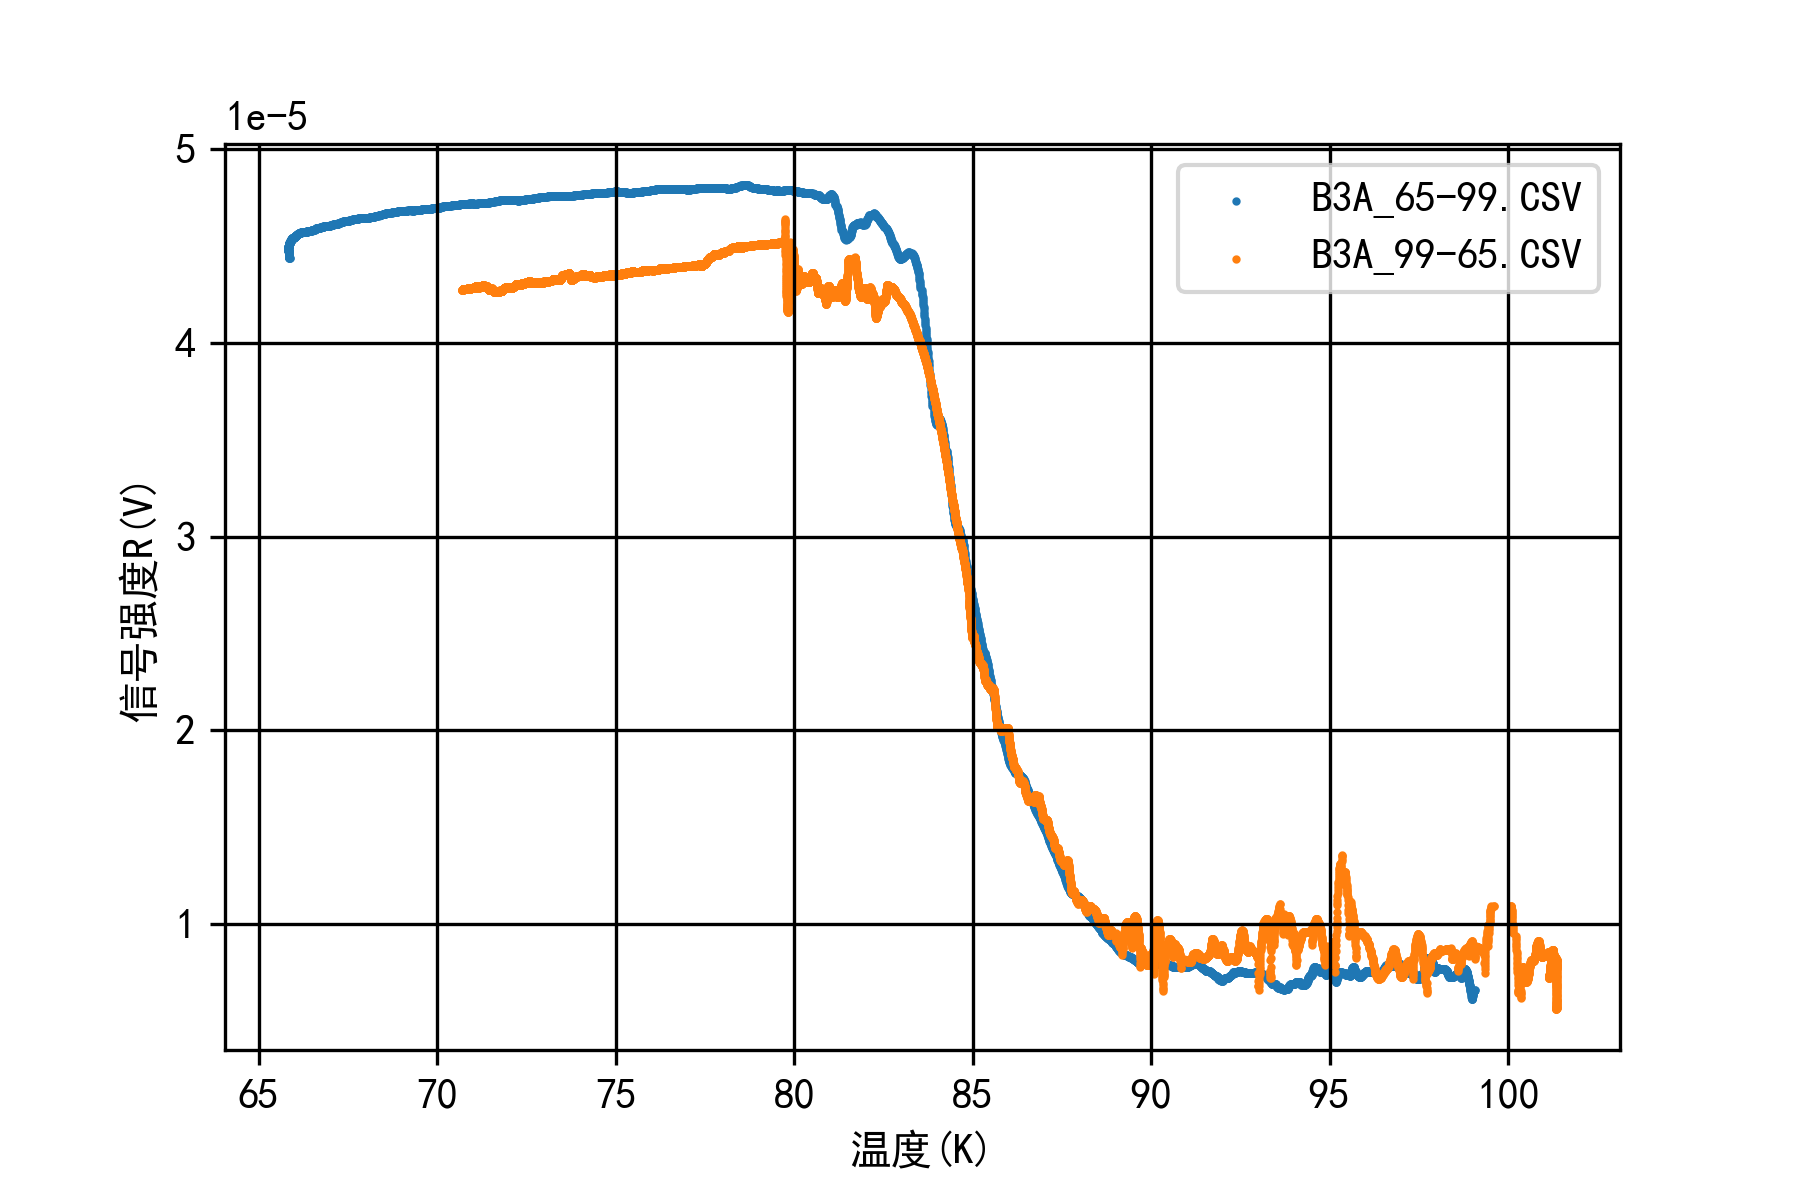
\includegraphics[width=0.9\linewidth]{./png/6.png}
			\caption{设置电流为3A}
		\end{minipage}
		\quad
		\begin{minipage}[t]{0.6\linewidth}
			\centering
			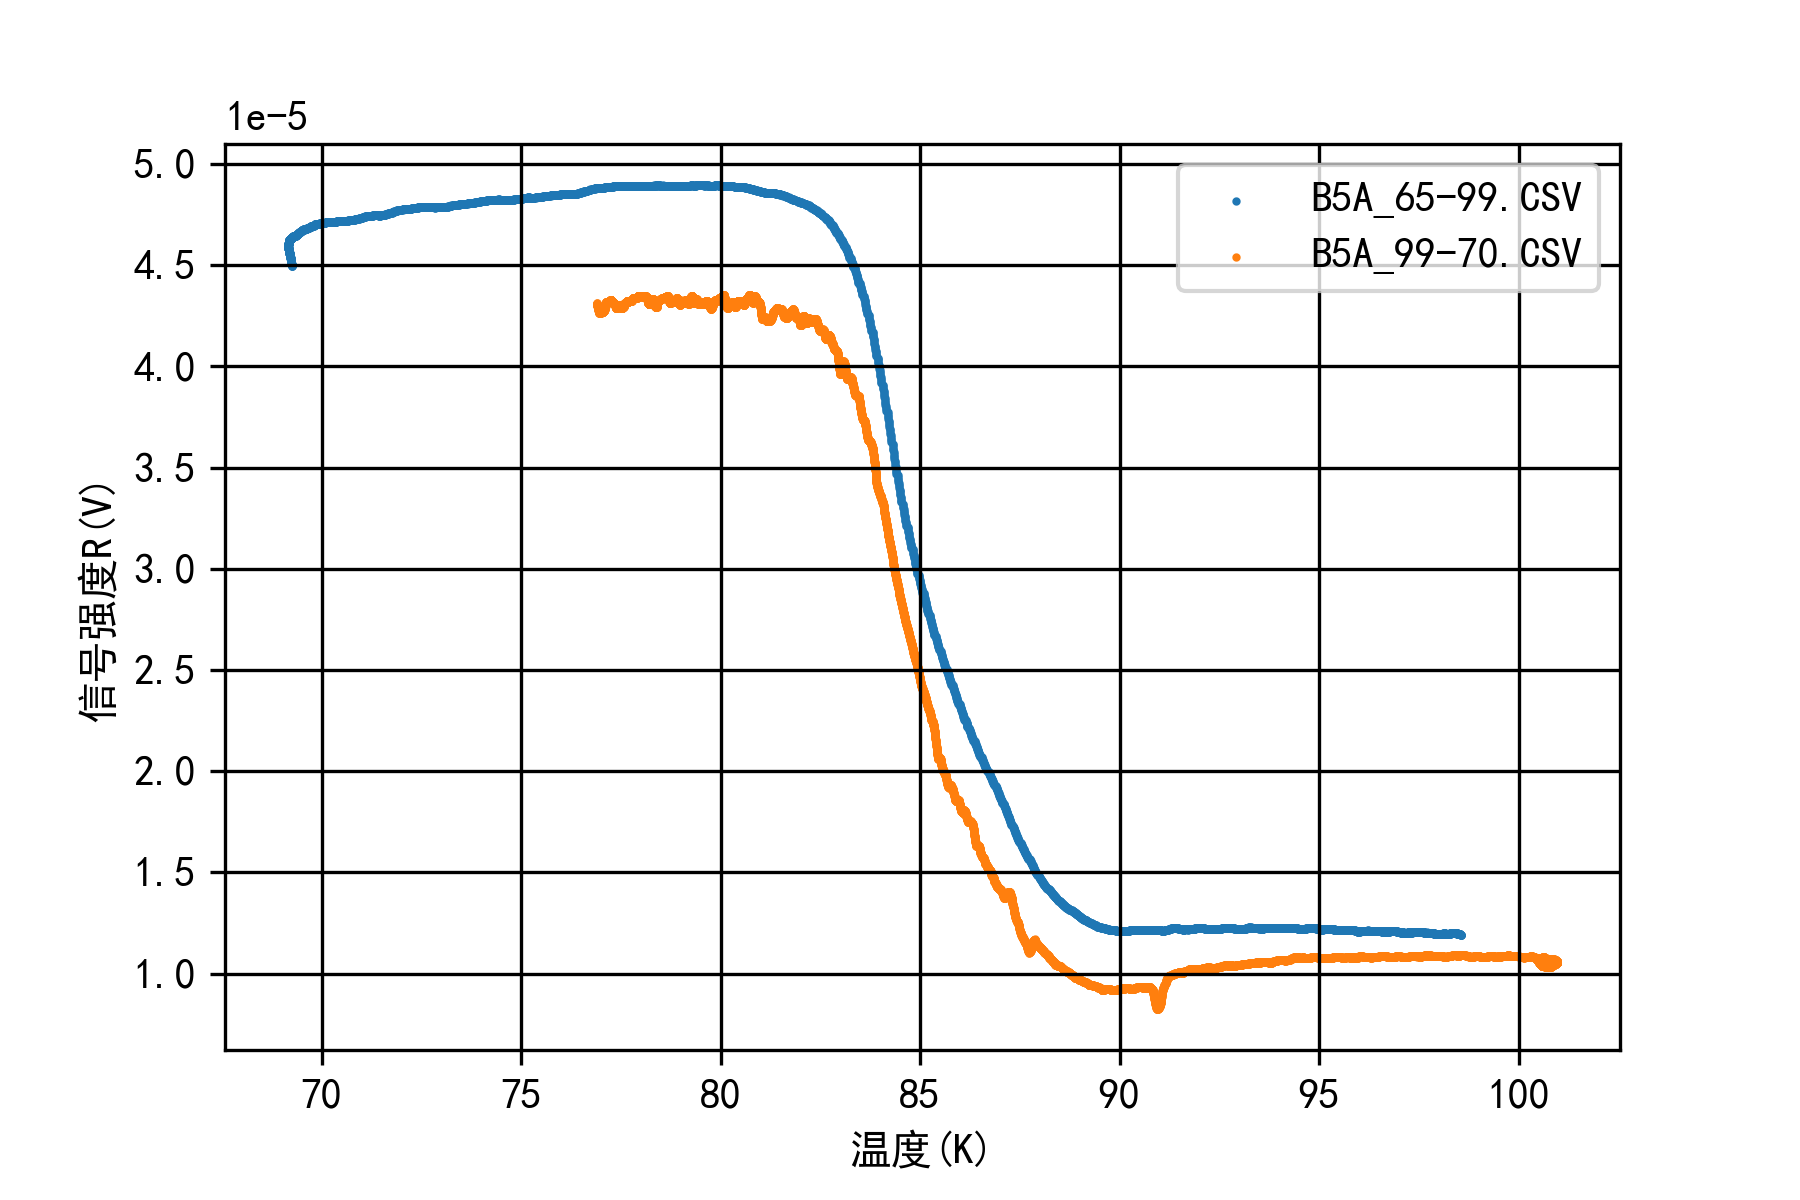
\includegraphics[width=0.9\linewidth]{./png/8.png}
			\caption{设置电流为5A}
		\end{minipage}
	\caption{在同一磁场设置下的升温降温记录情况,蓝色是升温曲线,黄色是降温曲线}
	
\end{figure}
\paragraph{}样品内部线圈可能正接,对比的电压信号值可能会与实例相反,同时我们无法与标准样品的磁化率做比较
故我们只能讨论其变化趋势\\
\paragraph{}磁场为0时,降温曲线和升温曲线在正常态下能达到重合,超导转变温度也基本一致,但在超导转变后,温度低于83K后相差逐渐增大,最后磁化率曲线随着降温趋于平稳,差值稳定。\\
\paragraph{}磁场电流设置为3A时,降温曲线和升温曲线在正常态下能达到重合,(此处降温曲线波动较大,可能是记录分辨率问题)超导转变温度也基本一致,在超导转变过程中,曲线能达到重合。但在超导转变后,温度低于84K后相差逐渐增大,最后随着降温,差值稳定。\\
\paragraph{}磁场电流设置为5A时,降温曲线和升温曲线在正常态下就有所区别,有一定差值。超导转变温度基本一致,在超导转变过程中和在超导转变后,温度低于83K后相差逐渐增大,最后随着降温,差值稳定。
\paragraph{}
从磁场电流设置为3A的图像可以看出,升温和降温过程基本重叠,而我们分析磁场设置为0A电流的数据以及
\paragraph[short]{原因分析:}   
在准静态的测量中,升温测量与降温测量的数据点十分接近,温差在0.1摄氏度
之内,说明超导过程与材料的温度变化趋势基本无关,而主要的影响因素还是具体的温度。而连续进行的
升温降温测量中升温测量会导致转变温度降低,而降温测量会导致转变温度升高,且多次测量后,升温的
转变温度区间大约在83-84摄氏度之间,与准静态测量的转变温度约差1摄氏度,而降温过程中转变温度区
间大约在86-88摄氏度之间,测量的随机误差较大,与准静态测量的转变温度约差2-3摄氏度,主要原因在
于热滞效应,此次数据是用的Pt1000温度传感器的阻值,而Pt1000附在了包裹材料的石墨外,所以温度
的响应较慢。如果能得到具体的厚度以及导热率可以用固体的热传导公式:$Q =\frac{\kappa S \Delta T}{L} $ 更加具体的建模标定
出样品的温度。同时,在升降温的过程中由于降温时几乎无法用PID控制降温速率,所以导致降温的速度
先快后慢,导致了转换温度的误差较大,而升温时速率较为平缓,与准静态的情况符合较好,误差在1摄氏
度之内
\paragraph*{}超导体具有零电阻效应和迈斯纳效应。本实验观察迈斯纳效应即在磁场强度低于临界值的情况下,磁力线无法穿过超导体,超导体内部磁场为零的现象。
不同磁场大小下,分别升温和降温的临界温度近似相同,而磁化率大小有区别。原因可能是样品并非理想第二类超导体。晶阵缺陷的存在,阻碍着磁通线的运动。
因此,可以把它们看作是一些对磁通线运动产生钉扎作用的钉扎体。只有体内组分均匀分布,不存在各种晶体缺陷,其磁化行为才呈现完全可逆,称为理想第二类超导体。


\subsubsection{本实验如何判断待测样品是否超导?提示:超导体的两个基本特性是
	什么?}
	\paragraph{答:} 超导的两个特性有
	\begin{enumerate}
		\item 超导材料处于超导态时电阻为零,能够无损耗地传输电能。如果用磁场在超导环中引发感应电流,这一电流可以毫不衰减地维持下去.
		\item 超导材料处于超导态时,只要外加磁场不超过一定值,磁力线不能透入,超导材料内的磁场恒为零.
	\end{enumerate}	
	
\subsubsection{本实验如何判断待测样品的超导态是否热力学状态? }
\paragraph{答:} 在本次实验中我们使用的是
\subsubsection{在磁化率定标前,如何把测量次级线圈的电压信号转换为磁化率(相同的量纲)}

	

% \newpage

\appendix
\begin{equation}
	\dfrac{a}{b} 
\end{equation}

\section{贡献说明}


\end{document}
